% !TeX program = xelatex
% T1 -- Food Analyzer final report, prepared 19 September 2026.
% Based directly on the course-supplied REPORT_TEMPLATE.tex.
% Retains its section hierarchy, A4 geometry, blue headings, code style,
% required deliverables, running furniture and bibliography structure.
% Use XeLaTeX or LuaLaTeX to preserve the members' Azerbaijani names.
\documentclass[11pt,a4paper]{article}
\usepackage[dvipsnames]{xcolor}
\usepackage[margin=2.2cm,headheight=15pt]{geometry}
\usepackage{fontspec}
\setmainfont{Times New Roman}
\setsansfont{Arial}
\setmonofont{Courier New}[Scale=0.82]
\usepackage[final,protrusion=true,expansion=false]{microtype}
\usepackage{amsmath,amssymb,graphicx,booktabs,array,tabularx,ragged2e}
\usepackage{enumitem}
\usepackage{multicol}
\usepackage[parfill]{parskip}
\usepackage{listings}
\usepackage[most]{tcolorbox}
\usepackage{titlesec,fancyhdr,lastpage}
\usepackage{tikz}
\usetikzlibrary{arrows.meta,positioning,fit,backgrounds}
\usepackage{xurl}
\usepackage[hidelinks]{hyperref}
\definecolor{accent}{HTML}{0B3D91}
\definecolor{soft}{HTML}{F2F4F8}
\definecolor{deliver}{HTML}{E8F0FE}
\definecolor{deliverframe}{HTML}{1A56DB}
\definecolor{probe}{HTML}{FFF8E1}
\definecolor{probeframe}{HTML}{B45309}
\definecolor{codegreen}{rgb}{0,0.55,0}
\definecolor{codegray}{rgb}{0.4,0.4,0.4}
\definecolor{codepurple}{rgb}{0.55,0,0.78}
\definecolor{backcolour}{rgb}{0.97,0.97,0.97}
\newcommand{\teamname}{T1}
\newcommand{\topicchoice}{Topic 2 -- AI Food Analyzer}
\newcommand{\reportdate}{19 September 2026}
\newcommand{\member}[2]{\textbf{#1} (#2)}
\newcommand{\repolink}{\href{https://github.com/Gunas12/Food_Analyzer}{github.com/Gunas12/Food\_Analyzer}}
\newcommand{\coursecode}{AI-ENG-110}
\newcommand{\coursename}{Software Engineering}
\newcommand{\institution}{AI Academy, National AI Center}
\newcommand{\semester}{Spring 2026}
\newcommand{\code}[1]{\texttt{\detokenize{#1}}}
\newcommand{\evidence}[1]{\par{\footnotesize\color{codegray}\textit{Repository evidence:} #1}\par}
\newcolumntype{Y}{>{\RaggedRight\arraybackslash}X}
\newtcolorbox{deliverbox}{colback=deliver,colframe=deliverframe,boxrule=0.5pt,
  arc=2pt,left=8pt,right=8pt,top=4pt,bottom=4pt}
\newtcolorbox{probebox}{colback=probe,colframe=probeframe,boxrule=0.5pt,
  arc=2pt,left=8pt,right=8pt,top=4pt,bottom=4pt}
\titleformat{\section}{\Large\bfseries\color{accent}}{\thesection.}{0.6em}{}
\titleformat{\subsection}{\large\bfseries\color{accent}}{\thesubsection}{0.5em}{}
\titlespacing*{\section}{0pt}{11pt}{5pt}
\titlespacing*{\subsection}{0pt}{8pt}{4pt}
\setlength{\parskip}{4pt}
\setlist{leftmargin=1.4em,itemsep=3pt,topsep=3pt}
\setcounter{tocdepth}{2}
\emergencystretch=3em
\lstdefinestyle{python}{language=Python,backgroundcolor=\color{backcolour},
  commentstyle=\color{codegreen},keywordstyle=\color{accent},
  numberstyle=\tiny\color{codegray},stringstyle=\color{codepurple},
  basicstyle=\ttfamily\footnotesize,breaklines=true,keepspaces=true,
  numbers=left,numbersep=6pt,tabsize=2,frame=single,framerule=0.4pt,
  rulecolor=\color{black!30},showstringspaces=false}
\hypersetup{colorlinks=true,linkcolor=NavyBlue,urlcolor=NavyBlue,citecolor=NavyBlue,
  pdftitle={T1 -- Food Analyzer Final Project Report},pdfauthor={Team T1}}
\pagestyle{fancy}
\fancyhf{}
\fancyhead[L]{\small\textit{\coursecode\ -- Final Report -- \teamname}}
\fancyhead[R]{\small\textit{\semester}}
\fancyfoot[L]{\footnotesize\textit{\institution}}
\fancyfoot[R]{\small Page \thepage\ of \pageref{LastPage}}
\renewcommand{\headrulewidth}{0.4pt}
\renewcommand{\footrulewidth}{0.4pt}
\begin{document}

% Planned page 1: title, summary, contents.
\begin{center}
{\small \institution\\[0.2em]\coursecode\ -- \coursename\ -- \semester}\\[0.8em]
{\Large\bfseries\color{accent} Final Project Report}\\[0.3em]
{\LARGE\bfseries\topicchoice}\\[0.4em]
\rule{0.85\textwidth}{0.6pt}
\end{center}
\begin{tabularx}{\textwidth}{@{}lYlY@{}}
\textbf{Team:} & \teamname & \textbf{Date:} & \reportdate\\
\textbf{Repo:} & \repolink & \textbf{Tag:} & \texttt{v1.0-final}\\
\textbf{Snapshot:} & \code{acce4e7} & \textbf{Branch:} & \code{main}\\
\end{tabularx}
\vspace{0.15em}
{\small\noindent
\begin{tabularx}{\linewidth}{@{}lYY@{}}
\textbf{Members:} & \member{Günəş Məmmədova}{\href{https://github.com/Gunas12}{@Gunas12}}
  & \member{Esmira Məmmədova}{\href{https://github.com/EsmiraMammadli}{@EsmiraMammadli}}\\
& \member{Əli Muradov}{\href{https://github.com/Ali-Muradov}{@Ali-Muradov}}
  & \member{Pünhan Mürsəlov}{\href{https://github.com/Punhan0}{@Punhan0}}\\
\end{tabularx}}

\section*{Executive Summary}
\addcontentsline{toc}{section}{Executive Summary}
Food Analyzer converts a meal photograph into estimated ingredients, portion sizes and a calorie/macronutrient breakdown through a browser interface, HTTP API and command-line entry point.
Team T1 built the configuration, validation, orchestration, persistence and testing layers around the supplied, unchanged \code{ai/} contract.
Nutrition lookups combine \code{asyncio.gather()}, a configurable semaphore with a default limit of ten, and \code{asyncio.to_thread()} to overlap synchronous provider calls.
The saved synthetic benchmark reports 1.517 seconds sequentially and 0.154 seconds concurrently, with a reported 9.9-fold speedup for ten simulated 150-millisecond lookups.
Bounded provider-error retries, a thread-safe 24-hour cache and partial-result handling support recovery, while a historical test log records 143 passing tests and 97\% coverage of \code{src/}.
The main limitation is that missing nutrition is represented as zero without an explicit completeness flag, so successful delivery does not guarantee complete or accurate nutritional data.

\section*{Contents}
{\footnotesize
\setlength{\parskip}{0pt}
\begin{multicols}{2}
\makeatletter
\@starttoc{toc}
\makeatother
\end{multicols}}

\clearpage
% Planned page 2.
\section{Project Overview}
\subsection{Problem framing \& scope}
Estimating a meal's nutritional content manually requires identifying ingredients, estimating portions and finding compatible nutrition records. Food Analyzer accepts a JPEG or PNG, asks a vision-language model for ingredient names, grams and confidence values, and combines per-100-gram nutrition facts into per-ingredient rows and meal totals. The estimates depend on both visual recognition and the selected nutrition match; the software does not establish a measured ground truth for a meal.

The browser page at \code{/} submits an image to \code{POST /analyze}. The HTTP response is a serialized \code{AnalysisRecord} containing an identifier, timestamp, image path, recognition flag, ingredient rows and totals. \code{GET /analyses/{analysis_id}} retrieves one saved record, and \code{GET /health} returns a simple status object. The CLI command \code{python -m foodanalyzer analyze <path>} delegates to \code{src.cli}, prints a table and persists the analysis. The original \code{demo_ai.py --offline} remains a separate, synchronous demonstration using filename-based fake recognition and fixed nutrition values.

The current snapshot integrates the team's pipeline into both API and CLI paths. It does not implement authentication, a history-list API, a global request budget or an explicit indication that nutrition is incomplete. These are implementation gaps, not evidence of a recorded team decision to drop requirements. The README documents a Render deployment and includes screenshots; its current availability was not probed for this report. Saved JSON responses provide historical examples, not a fresh deployment verification.

\subsection{Provider choice and the AI module contract}
The documented project stack is Gemini for image understanding and USDA FoodData Central for nutrition lookup. \code{Settings} defaults to \code{gemini} and \code{gemini-2.0-flash}; \code{requirements.txt} enables \code{google-genai==1.0.0}. The supplied package also contains Anthropic and OpenAI adapters, whose SDK dependencies are commented out. No embedding or web-search provider participates in the implemented food-analysis flow. Gemini image input and USDA data access are documented in the official references~\cite{gemini,usda}.

There is configuration drift: \code{.env.example} still selects \code{anthropic} and \code{claude-sonnet-4-6}, and the supplied VLM factory defaults to Anthropic when its process environment is unset. The API calls \code{load_dotenv()}, whereas the CLI only constructs \code{Settings}; it does not copy those parsed values into the process environment read by the provider factory. Consequently, the documented Gemini configuration must not be presented as proof of the provider/model used in a particular saved run. The effective provider and model used for the submitted demonstration are not recorded in the inspected repository evidence, so this report leaves that run-specific claim unverified.

The team did not modify the public interface of the provided \code{ai/} package: comparison with the repository's initial commit \code{b976c0d} shows no changes in that directory or in \code{tests/test_ai_smoke.py}. This establishes continuity within the available repository history, not an independent comparison with an external distribution archive. Calls use \code{identify_ingredients}, \code{NutritionProvider.lookup} and \code{compute_totals}; the provider adapters remain part of the supplied code.

\evidence{\code{TOPIC.md}; \code{README.md}; \code{src/api.py}; \code{src/cli.py}; \code{foodanalyzer/__main__.py}; \code{src/config.py}; \code{ai/providers/factory.py}; Git comparison \code{b976c0d..acce4e7}.}

\clearpage
% Planned page 3.
\section{Architecture}\label{sec:arch}
\subsection{Module map}
\begin{center}
\resizebox{0.98\textwidth}{!}{%
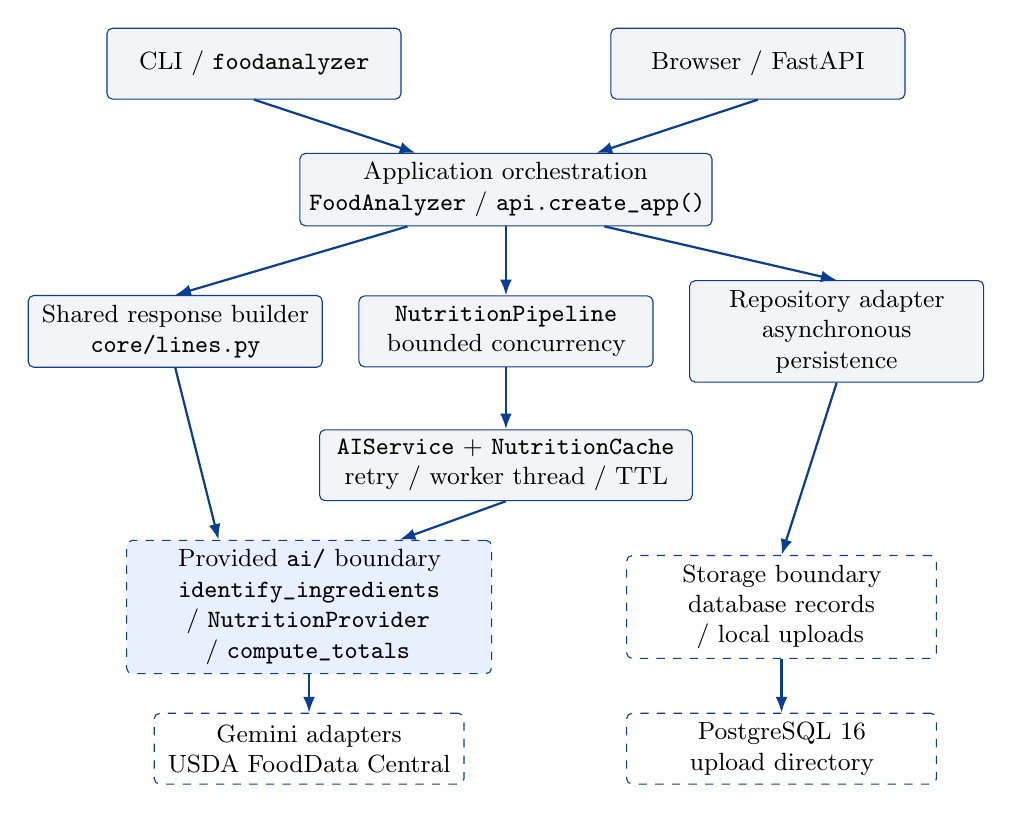
\begin{tikzpicture}[
  box/.style={draw=accent,rounded corners=2pt,fill=soft,align=center,
    text width=3.5cm,minimum height=0.9cm,font=\small},
  boundary/.style={box,dashed,fill=deliver,text width=4.4cm,minimum height=1.15cm},
  external/.style={box,dashed,fill=white,text width=3.7cm},
  flow/.style={-{Latex[length=2mm]},thick,draw=accent},
  every node/.style={font=\small}]
\node[box] (cli) at (-3.2,0) {CLI / \code{foodanalyzer}};
\node[box] (web) at (3.2,0) {Browser / FastAPI};
\node[box,text width=5.0cm] (orchestrator) at (0,-1.6)
  {Application orchestration\\\code{FoodAnalyzer} / \code{api.create_app()}};
\node[box] (builder) at (-4.2,-3.4)
  {Shared response builder\\\code{core/lines.py}};
\node[box] (pipeline) at (0,-3.4)
  {\code{NutritionPipeline}\\bounded concurrency};
\node[box] (repo) at (4.2,-3.4)
  {Repository adapter\\asynchronous persistence};
\node[box,text width=4.5cm] (service) at (0,-5.1)
  {\code{AIService} + \code{NutritionCache}\\retry / worker thread / TTL};
\node[boundary] (ai) at (-2.5,-6.9)
  {Provided \code{ai/} boundary\\\code{identify_ingredients} / \code{NutritionProvider} / \code{compute_totals}};
\node[boundary,fill=white,text width=3.7cm] (storage) at (3.5,-6.9)
  {Storage boundary\\database records / local uploads};
\node[external] (providers) at (-2.5,-8.7)
  {Gemini adapters\\USDA FoodData Central};
\node[external] (db) at (3.5,-8.7)
  {PostgreSQL 16\\upload directory};

% Every connector begins and ends on a node border. The fan-out anchors keep
% all routes in the whitespace between rows, away from every module frame.
\draw[flow] (cli.south) -- ([xshift=-1.15cm]orchestrator.north);
\draw[flow] (web.south) -- ([xshift=1.15cm]orchestrator.north);
\draw[flow] ([xshift=-1.25cm]orchestrator.south) -- (builder.north);
\draw[flow] (orchestrator.south) -- (pipeline.north);
\draw[flow] ([xshift=1.25cm]orchestrator.south) -- (repo.north);
\draw[flow] (pipeline.south) -- (service.north);
\draw[flow] (builder.south) -- ([xshift=-1.15cm]ai.north);
\draw[flow] (service.south) -- ([xshift=1.15cm]ai.north);
\draw[flow] (repo.south) -- (storage.north);
\draw[flow] (ai.south) -- (providers.north);
\draw[flow] (storage.south) -- (db.north);
\end{tikzpicture}}
\end{center}
{\small Arrows denote calls or dependencies, not an execution schedule. The CLI and API have separate entry points but share response construction, nutrition services and supplied AI contracts. Database records pass through the repository; uploaded files remain on the local storage path.}

{\small
\begin{tabularx}{\textwidth}{@{}p{4.1cm}Y@{}}
\toprule\textbf{Module group} & \textbf{Responsibility}\\\midrule
\code{config.py}, \code{wiring.py} & Typed settings, logging setup and the CLI composition root.\\
\code{api.py}, \code{cli.py} & Transport-specific input, orchestration and responses; the API does not call \code{FoodAnalyzer}.\\
\code{core/analyzer.py}, \code{core/lines.py} & CLI analysis sequence and shared construction of ingredient rows/totals.\\
\code{services/}, \code{concurrency/} & Provider retries in worker threads, TTL cache and bounded concurrent nutrition lookup.\\
\code{models.py}, \code{storage/} & Application records, JSON conversion and asynchronous persistence.\\
\code{ai/}, \code{static/} & Supplied provider contract/calculation and the team's browser upload interface, respectively.\\\bottomrule
\end{tabularx}}
The service and shared totals helper cross the AI boundary; \code{Repository} crosses the database boundary. Switching among supplied VLMs can use environment/dependency changes without editing business logic, provided the selected SDK is installed and the effective environment is correct. The diagram does not imply a single shared API/CLI orchestration method.

\clearpage
% Planned page 4.
\subsection{OOP design \& key abstractions}
\code{NutritionPipeline} composes a \code{NutritionProvider}, \code{AIService}, \code{NutritionCache} and semaphore. Provider lookup, retry policy and cache lifetime remain separate responsibilities. A pipeline is not a specialized cache or provider, so inheritance between those classes would misrepresent their relationship. Replacing an injected collaborator allows a test to control failures, cache state or scheduling without invoking an external service.

The following seven lines are copied from \code{src/wiring.py}. They show the team's actual composition rather than an invented storage interface:
\begin{lstlisting}[style=python]
    cache = NutritionCache(ttl_seconds=settings.nutrition_cache_ttl_seconds)
    pipeline = NutritionPipeline(
        nutrition_provider,
        cache=cache,
        ai_service=ai_service,
        max_parallel=settings.max_parallel,
    )
\end{lstlisting}

\code{NutritionProvider} is the supplied abstract base class with a synchronous \code{lookup} contract; \code{USDAProvider} and several test fakes subclass it. Retaining this contract avoids changing the frozen package. A structural protocol could describe compatible objects, but the team did not introduce one: the benchmark's fake happens to satisfy the lookup surface without inheriting the ABC. \code{AIService} and \code{NutritionCache} need no artificial base classes; injected sleep and clock callables supply their testing extension points.

\code{FoodAnalyzer} composes service, pipeline and repository. \code{Components}, a dataclass in \code{wiring.py}, groups constructed dependencies; it is not a transport response. \code{create_app()} provides separate injection points for provider factories, repository, service and cache. This makes API tests independent of the real SDKs and PostgreSQL, while preserving the production call structure.

\subsection{Data flow across module boundaries}
\begin{enumerate}
\item Input validation yields a filesystem path. \code{AIService.identify_ingredients()} delegates to the supplied VLM layer and returns \code{list[Ingredient]}. Each frozen Pydantic ingredient has a nonblank name, nonnegative grams and confidence in the range 0--1.
\item \code{NutritionPipeline.lookup()} receives those ingredients and returns \code{dict[str, NutritionFacts]}. Facts are immutable, per-100-gram Pydantic objects. Cache/grouping keys are normalized, but the returned mapping preserves original ingredient spellings for the calculator's case-sensitive lookup.
\item \code{build_ingredient_lines()} produces \code{list[IngredientLine]} and \code{MealTotals}. It scales successful facts by grams/100, keeps failed ingredients with zero macros, and obtains aggregate values through \code{ai.compute_totals()}.
\item API and analyzer create \code{AnalysisRecord} directly. \code{AnalysisResult} and \code{AnalysisRecord.from_result()} also exist and are tested, but are not the active orchestrators' intermediate representation.
\item \code{Repository.save()} converts model fields to JSON-compatible dictionaries, commits the row, refreshes it and returns a record with identifier/timestamp. Retrieval validates stored JSON back into application models; the API serializes the record using \code{model_dump} with \code{mode="json"}.
\end{enumerate}
The application models use \code{extra="forbid"}, but their numeric fields do not repeat all of \code{Ingredient}'s bounds. Dictionaries intentionally cross the nutrition and serialization boundaries; an assertion that no dictionaries cross modules would be false. Model separation permits response/storage evolution without modifying the supplied AI types~\cite{pydantic}.

\evidence{\code{src/wiring.py}; \code{src/models.py}; \code{src/core/lines.py}; \code{src/storage/repository.py}; \code{ai/schemas.py}; \code{ai/nutrition.py}.}

\clearpage
% Planned page 5.
\section{Concurrency \& Performance}\label{sec:concurrency}
\subsection{Why this concurrency model}
Nutrition lookups are independent synchronous operations whose network waiting can overlap. \code{asyncio.gather()} schedules one coroutine per distinct normalized ingredient; \code{asyncio.to_thread()} runs each actual synchronous call outside the event-loop thread. The semaphore gates entry to a lookup/retry sequence, including its backoff sleeps. Async orchestration fits the HTTP application and avoids rewriting the supplied provider API; it still uses worker threads for the blocking work~\cite{asyncio,semaphore}.

The default \code{max_parallel=10} matches the topic's suggested bound, not a measured optimum. One pipeline instance shares its semaphore across its batches on one event loop. Crucially, \code{POST /analyze} constructs a new pipeline for each request: the API shares its cache and service, but \emph{not} an application-wide semaphore. Simultaneous requests can therefore exceed ten aggregate provider calls. Deduplication is guaranteed within a batch, including when TTL is zero; separate batches can independently fetch the same miss.

VLM recognition precedes nutrition lookup; record construction and totals are synchronous, and database operations are awaited afterward. Image-file writing in the API is synchronous too. A bound of one serializes cache misses; a much larger bound increases resource/provider pressure without guaranteeing throughput. A provider shared by worker threads must be thread-safe, or that pipeline should use \code{max_parallel=1}. This does not globally serialize separate API pipelines.

\subsection{Sequential-vs-concurrent benchmark}
\begin{center}\small
\begin{tabular}{@{}lrrrr@{}}
\toprule
\textbf{Saved synthetic workload} & $N$ & \textbf{Seq. (s)} & \textbf{Conc. (s)} & \textbf{Speedup}\\\midrule
150 ms per fake lookup & 10 & 1.517 & 0.154 & 9.9$\times$\\\bottomrule
\end{tabular}
\end{center}
These are the values in \code{artefacts/benchmark.txt}, introduced at \code{3ff73fb}. The README instead prints 1.518/0.153 seconds; the saved raw output is used here without combining the two runs. \code{scripts/bench.py} uses ten distinct names, a blocking fake provider, monotonic wall-clock timing, sequential service calls and then a pipeline with a fresh empty cache and limit ten. It excludes VLM work, real USDA traffic, database writes and HTTP overhead. No benchmark was rerun for this report.

The measured times are close to the simulated 1.5-second sequential and 0.15-second concurrent latency floors. The small excess is consistent with execution/scheduling overhead, but no profiler identifies its breakdown. The printed speedup uses unrounded internal times. This single result does not establish an end-to-end speedup, statistical variability or the smallest profitable workload. The saved output does not record the benchmark machine/OS, Python version, run date, exact command or source commit; that omission limits independent timing reproduction and is stated rather than filled with invented metadata.

\subsection{Rate limit \& politeness}
The system has concurrency admission and exponential backoff, not a full requests-per-minute limiter. It has no token bucket, shared request budget, jitter or \code{Retry-After} interpretation. HTTP 429 is retried only when the provider converts it into \code{ProviderError}; the same wrapper handles other provider errors. There is no saved evidence of a real 429 experiment.

Event-gated tests exercise an explicit two-call overlap and bounds of one, two and three across batches. These verify scheduling correctness, not elapsed-time performance or a maximum live traffic burst. A production request budget and a shared API admission gate remain future work.
\evidence{\code{src/concurrency/pipeline.py}; \code{src/api.py}; \code{scripts/bench.py}; \code{artefacts/benchmark.txt}; \code{tests/test_pipeline.py}.}

\clearpage
% Planned page 6.
\section{Robustness \& Error Handling}\label{sec:robustness}
\subsection{Wrapping the AI module}
\code{AIService} implements retries manually, without \code{tenacity}. Only \code{ProviderError} is caught; with defaults there are three total attempts and two asynchronous delays of 0.5 and 1.0 seconds. More generally, delay after failed attempt $k$ is $b\,2^{k-1}$, for $k<m$, where $b$ is \code{base_delay} and $m$ is \code{max_attempts}. The final error is re-raised unchanged. Non-provider programming errors propagate immediately. The constructor rejects noninteger/boolean attempt counts, counts below one, and negative or nonfinite delays.

An injected asynchronous sleep enables deterministic retry tests. Cancellation during backoff is not swallowed. There is no independent service-level per-call deadline; the supplied USDA adapter sets a 10-second timeout on its HTTP request, which does not bound a complete analysis. Cancelling an awaiting coroutine also does not guarantee that an already-running blocking provider thread stops immediately.

The service logs start, retry and success at INFO with operation, attempt and delay values, omitting image paths and provider-error payloads. Pipeline exhaustion logs an ingredient name at WARNING without the exception payload. This protection is local: API exception handlers log raw provider exception text or include it in \code{extra}. Thus application-wide redaction cannot be claimed. \code{configure_logging()} now applies \code{LOG_LEVEL} and a timestamp/level/logger/message format; these are conventional text logs, not a comprehensive structured-event schema.

\subsection{Failure-mode analysis: exhausted ingredient lookup}
The repository's \code{test_provider_failure_preserves_other_results_and_logs_warning} scripts three \code{ProviderError} outcomes for ``unknown'' alongside successful rice and broccoli lookups. The service exhausts the three attempts using mocked sleep; the pipeline omits the failed key, preserves both successful facts, does not cache the failure and emits one warning. Assertions verify that the private error payload is absent and that the supplied calculator sums only the two successful 100-gram portions, yielding 260 kcal in this fake scenario.

At application level, \code{build_ingredient_lines()} retains an unsuccessful ingredient with zero macros. The API test \code{test_analyze_unknown_ingredient_still_returns_ok} verifies HTTP 200 for an all-missing-nutrition case, with \code{meal_recognized=true} and zero totals. Therefore lookup exhaustion is \emph{not} an HTTP 503 in this path. Exhausted VLM errors and failure to construct the nutrition provider have explicit 503 responses; storage errors and other uncaught failures have no custom mapping. The CLI catches image-validation errors as exit code 2, while provider/storage failures propagate. These are code/test-supported behaviors, not a claimed live outage investigation.

\subsection{Input validation}
{\small
\begin{tabularx}{\textwidth}{@{}p{2.6cm}Y@{}}
\toprule\textbf{Boundary} & \textbf{Implemented rule and response}\\\midrule
CLI/file & Existing nonempty file; JPEG/PNG extension and magic prefix; default maximum 5 MiB. Errors include ``file not found'', ``file is empty'' and ``file too large'', printed with \code{error:} and exit 2 after setup succeeds.\\
HTTP upload & Requires \code{file}; checks JPEG/PNG content type, nonempty content, configured size and magic bytes; explicit failures return 400. UUID filenames avoid trusting the client path. Missing multipart input/type-invalid route parameters use framework validation (422)~\cite{fastapi}.\\
VLM output & Parses a JSON object and validates the response envelope and bounded \code{Ingredient} fields; malformed/schema-invalid responses become \code{ProviderError}. An unrecognized meal yields an empty list.\\
Environment & Pydantic validates provider/log-level enums, ports 1--65535, positive parallel/image limits and nonnegative TTL. Keys are optional in settings but required when real providers are constructed.\\\bottomrule
\end{tabularx}}
Magic-byte checks are not complete image decoding. The API reads the full upload before applying its byte limit; this is not a streaming memory cap. Signature-valid but corrupted images and very large inputs remain limitations.

\clearpage
% Planned page 7.
\section{Storage \& Caching}\label{sec:storage}
\subsection{Schema}
The deployed configuration targets PostgreSQL through SQLAlchemy's asynchronous engine and \code{asyncpg}. Offline repository tests substitute in-memory SQLite; SQLite is not the production database. The following table transcribes the actual ORM mapping, rather than presenting an unverified SQL migration. Async session/engine APIs are documented by SQLAlchemy~\cite{sqlalchemy}.

{\small
\begin{tabularx}{\textwidth}{@{}p{3.0cm}p{3.1cm}Y@{}}
\toprule\textbf{Column} & \textbf{ORM type} & \textbf{Meaning / constraints}\\\midrule
\code{id} & Integer & Primary key; autoincrement.\\
\code{created_at} & Timezone-aware DateTime & Nonoptional mapped field; Python UTC default evaluated on insert.\\
\code{image_path} & String & Required; references an image in the filesystem.\\
\code{meal_recognized} & Boolean & Required; Python default \code{True}.\\
\code{ingredients} & JSON & Required; ingredient dictionaries, default empty list.\\
\code{totals} & JSON & Required; macro dictionary, default empty dict.\\\bottomrule
\end{tabularx}}

\code{analysis_records} has no declared foreign keys or secondary indexes. \code{init_models()} invokes \code{metadata.create_all}; no versioned migration system is present. Defaults above are ORM-side values, not explicit database \code{server_default} declarations. \code{save()} commits and refreshes a row; \code{get()} returns a typed record or \code{None}; \code{list_recent()} sorts by timestamp and ID descending but has no list HTTP endpoint.

Ingredient estimates and derived macro totals are stored as an analysis snapshot; there are no embedding blobs. Raw provider responses, per-100-gram fact provenance and explicit missing-fact flags are not persisted. PostgreSQL is the history store, while uploaded bytes live under \code{uploads/}. Compose persists the database in \code{foodanalyzer_pgdata}, but defines no API upload volume, so stored paths can outlive image files when the API container is replaced.

\subsection{Caching policy}
\code{NutritionCache} stores immutable \code{NutritionFacts} in a process-local dictionary. The default TTL is 86,400 seconds; keys use \code{strip().casefold()}, preserving internal whitespace. A \code{threading.Lock} protects reads and writes, and \code{time.monotonic()} supplies expiry times through an injectable clock. At \code{now >= expires_at}, a get removes the stale entry and returns a miss. This lazy cleanup has no background sweep or capacity limit. Reads do not extend TTL; setting a value replaces it and resets expiry. Zero TTL disables retention.

The pipeline checks cache before acquiring the semaphore and again after entering it, preventing a redundant provider call when another operation filled the cache during the wait. Successful fetches populate the cache; failed fetches do not. Restarting a process loses it, and multiple processes have independent caches. Keys contain no provider/model/version information, and deduplication is not a cross-request single-flight mechanism. No demo cache-hit rate was saved, so this report does not infer one from correctness tests.

\section{Testing}\label{sec:testing}
\subsection{Strategy \& historical coverage}
The tests use fake VLM/nutrition providers, FastAPI \code{TestClient}, fake API repositories and SQLite-backed repository/analyzer fixtures. CLI wiring is monkeypatched; service retries use \code{AsyncMock}; clocks, thread IDs and event gates control time and concurrency. They do not need real provider responses to exercise these paths~\cite{pytest}.

\clearpage
% Planned page 8.
The committed \code{artefacts/coverage.txt} records the following historical run. It was added in \code{3ff73fb}, before later refactoring and logging/validation changes. In particular, its coverage table does not include the subsequently added \code{src/core/lines.py}. It must not be represented as coverage freshly measured at \code{acce4e7}.

\begin{center}\small
\begin{tabular}{@{}ll@{}}
\toprule\textbf{Saved result} & \textbf{Recorded value}\\\midrule
Execution environment & Windows; Python 3.13.15; pytest 9.1.1\\
Suite & 143 collected; 143 passed in 3.40 seconds\\
\code{src/} coverage & 97\%; 484 statements, 16 missed\\
Service/cache/pipeline & 100\% each in that saved run\\
Provided smoke suite & 29 passing cases in the saved output\\\bottomrule
\end{tabular}
\end{center}
\textbf{Tests and coverage were not rerun during this report-writing task.} The README also reports zero mypy errors, but there is no saved mypy transcript; \code{mypy.ini} suppresses errors under \code{ai.*}. No fresh type-check result is asserted. The report therefore labels 143 passing tests and 97\% coverage as historical evidence rather than validation tied to the final submission commit.

\subsection{Notable tests}
\begin{description}[style=nextline,leftmargin=0pt]
\item[Happy path.] \code{test_happy_path_recognized_meal} in \code{tests/test_analyzer.py} validates a temporary image, uses fake service/pipeline data, and persists a recognized meal through the real repository interface against SQLite. \code{test_result_is_persisted_and_retrievable} checks retrieval. This is an offline orchestration integration test, not a real-provider end-to-end run.
\item[Concurrency.] \code{test_sync_lookups_overlap_and_allow_event_loop_progress} holds two synchronous fake lookups behind a thread event. It checks two distinct worker threads, overlap and a responsive event loop before releasing them. Another test gates two batches and verifies bounds of one, two and three. Neither is a speed benchmark.
\item[Failure path.] The exhausted-ingredient scenario in Section~\ref{sec:robustness} checks partial success and safe service/pipeline logging. Additional tests verify recovery, original-error re-raising, cancellation during backoff and immediate propagation of \code{ValueError}, \code{TypeError} and \code{RuntimeError}.
\end{description}
Cache tests cover the exact TTL boundary, Unicode case folding, refresh, zero TTL, invalid configuration and 128 operations across eight threads. Pipeline tests check normalized duplicates, original-name/portion preservation, cache rechecks and retries after a previous batch failed. Gaps include live PostgreSQL/provider behavior, aggregate limits across API requests and post-refactor coverage; the current API tests also lack a dedicated spoofed-content-type/magic-byte regression case.

\section{Deployment \& Reproducibility}\label{sec:deploy}
\subsection{Docker image}
\code{Dockerfile} uses two \code{python:3.12-slim} stages, builds a virtual environment and copies it into a non-root runtime image~\cite{docker}. It copies \code{ai/}, \code{data/}, \code{src/} and \code{static/}, then runs Uvicorn on port 8000. The \code{foodanalyzer/} alias package, tests and benchmark script are not copied. Compose builds this API and starts \code{postgres:16-alpine}, waiting for the database health check. The repository-backed build/start command is \code{docker compose up --build}; shutdown is \code{docker compose down}. No saved final-image build, image size, digest or runtime transcript exists in the inspected evidence, and the Python patch version is not pinned; this report does not claim those missing measurements.

\clearpage
% Planned page 9.
\subsection{Configuration}
\code{Settings} reads environment variables and \code{.env}, ignores unknown fields and is cached by \code{get_settings()}. The table distinguishes its defaults from the supplied providers' direct environment reads. Pydantic's settings mechanism is documented separately~\cite{settings}.

{\footnotesize
\begin{tabularx}{\textwidth}{@{}p{5.15cm}Y@{}}
\toprule\textbf{Variable(s)} & \textbf{Default / behavior when absent}\\\midrule
\code{LLM_PROVIDER}, \code{LLM_MODEL} & Settings: Gemini / \code{gemini-2.0-flash}. Supplied factory: Anthropic; adapter model defaults differ. API loads dotenv into the process; CLI settings alone do not export it.\\
\code{GOOGLE_API_KEY}, \code{GEMINI_API_KEY} & Gemini checks these in order, then \code{LLM_API_KEY}. Missing all accepted keys raises \code{ProviderError} at construction.\\
\code{ANTHROPIC_API_KEY}, \code{OPENAI_API_KEY}, \code{LLM_API_KEY} & The selected Anthropic/OpenAI adapter uses its own key then \code{LLM_API_KEY}. No usable key causes \code{ProviderError}; settings themselves allow absent keys.\\
\code{NUTRITION_PROVIDER}, \code{USDA_API_KEY} & Provider defaults to \code{usda}; only USDA is shipped. A missing/empty USDA key prevents provider construction.\\
\code{DATABASE_URL} & If absent/empty, build \code{postgresql+asyncpg://} URL from the PostgreSQL fields below; an explicit URL wins.\\
\code{POSTGRES_USER}, \code{POSTGRES_PASSWORD}, \code{POSTGRES_DB} & \code{postgres}, \code{dev}, \code{foodanalyzer}; development defaults, not a production credential policy.\\
\code{POSTGRES_HOST}, \code{POSTGRES_PORT} & \code{localhost}, 5432; Compose sets API host to \code{db}. Port is constrained to 1--65535.\\
\code{LOG_LEVEL} & \code{INFO}; DEBUG/INFO/WARNING/ERROR accepted. API/CLI call \code{configure_logging()}.\\
\code{NUTRITION_CACHE_TTL_SECONDS} & 86400; integer at least zero, passed into the cache.\\
\code{MAX_PARALLEL} & 10; integer at least one, passed to each pipeline.\\
\code{MAX_IMAGE_SIZE_MB}, \code{UPLOAD_DIR} & 5 and \code{uploads}; size setting at least one, byte conversion uses $1024^2$.\\
\code{HTTP_PORT} & 8000 in settings, but current Docker/Uvicorn arguments and Compose ports are literal 8000; changing this variable alone does not change them.\\
\bottomrule
\end{tabularx}}

Before running Compose, the documented Gemini values must replace the Anthropic sample configuration. An explicit \code{DATABASE_URL} copied from \code{.env.example} still points to \code{localhost}, overriding Compose's \code{POSTGRES_HOST=db}; its host must match the deployment. For the CLI, provider values must be available in the process environment. The README's CLI ``offline'' label is inaccurate: this CLI constructs real providers and storage; \code{python demo_ai.py --offline} is the verified offline command. These discrepancies are reported, not modified.

\section{Limitations \& Future Work}\label{sec:limits}
\begin{itemize}
\item \textbf{Incomplete or inaccurate nutrition.} Missing facts appear as zero, and the supplied USDA extraction selects a top match without unit-aware energy selection. Saved examples are not accuracy validation. Add completeness/provenance fields and measured quality checks; resolve supplied-package issues through its owner.
\item \textbf{Request control.} No service-wide deadline or global rate budget exists, and API semaphores are per request. Add shared admission, bounded deadlines and retry jitter while accounting for continuing worker threads after cancellation.
\item \textbf{Cache lifetime.} Cache entries are process-local, unbounded and lazily removed; simultaneous misses may repeat across batches. Add capacity limits, provider-aware keys and shared in-flight lookup coordination.
\item \textbf{Operational consistency.} Environment defaults differ, uploads lack a persistent volume, and orchestration remains split between API and CLI. Unify configuration and lifecycle management and verify deployment with the final commit.
\item \textbf{Validation and observability.} Uploads are fully buffered and only signature-checked; API logging can expose provider details. Add bounded streaming, complete image validation and consistent redaction, with regression and load tests.
\end{itemize}

\clearpage
% Planned page 10.
\section{Tools \& Acknowledgements}\label{sec:tools}
The course-provided \code{ai/} package remained a frozen external contract. Codex assisted User \#3 with the service wrapper, TTL cache, concurrent pipeline, related tests and explanations; it also inspected repository evidence, drafted this report and diagram, and compiled the template-based PDF. It did not rerun tests, call live providers or build Docker images. The team remains responsible for the final work; individual review/adaptation confirmations and any additional assistant use must be declared by the relevant members.

\section{Team Contributions}\label{sec:team}
Names and accounts follow the supplied team list. Responsibilities combine file-level Git history with \code{report/CONTRIBUTION_STATEMENT.md}; they describe primary areas, not sole authorship or effort percentages.

{\small
\begin{tabularx}{\textwidth}{@{}p{3.7cm}Y@{}}
\toprule\textbf{Member / account} & \textbf{Repository-supported responsibilities}\\\midrule
\shortstack[l]{Günəş Məmmədova\\\code{@Gunas12}} & Models, settings, validation, composition root, CLI, Docker integration and documentation.\\[2pt]
\shortstack[l]{Esmira Məmmədova\\\code{@EsmiraMammadli}} & FastAPI, static UI, benchmark, shared response builder, logging and upload checks.\\[2pt]
\shortstack[l]{Əli Muradov\\\code{@Ali-Muradov}} & Retry service, TTL cache, bounded concurrent pipeline and their offline tests.\\[2pt]
\shortstack[l]{Pünhan Mürsəlov\\\code{@Punhan0}} & Async repository, persistence tests, storage dependencies and typing fixes.\\\bottomrule
\end{tabularx}}

Raw commit counts are not treated as effort shares. Signatures remain administrative submission items. The statement names \code{v1.0-final}, but that tag is absent locally, so the report identifies reviewed commit \code{acce4e7} separately.

\appendix
\section{Appendix --- Reproducing the benchmark}\label{sec:repro}
From the repository root, this offline command runs ten fake 150 ms lookups with parallel limit ten; it needs no API key or database.
\begin{lstlisting}[style=python,language=bash,numbers=none]
# PowerShell: make repository imports visible.
$env:PYTHONPATH="."
python scripts/bench.py
\end{lstlisting}
This reproduces the workload definition, not a guaranteed time. Future runs should preserve the environment, revision and raw output. Historical coverage used \code{pytest --cov=src --cov-report=term-missing}; it was not rerun here.

\clearpage
\begin{thebibliography}{10}
\addcontentsline{toc}{section}{References}
\bibitem{repo} Team T1. \textit{Food Analyzer source and project evidence}, reviewed commit \code{acce4e71798492ad4676f7967a0b47635fccd61a}. \url{https://github.com/Gunas12/Food_Analyzer/tree/acce4e71798492ad4676f7967a0b47635fccd61a}. Saved measurements: \code{artefacts/benchmark.txt} and \code{artefacts/coverage.txt}; ownership: \code{report/CONTRIBUTION_STATEMENT.md}.
\bibitem{asyncio} Python Software Foundation. \textit{Coroutines and Tasks}: concurrent gathering and running blocking calls in threads. \url{https://docs.python.org/3/library/asyncio-task.html}.
\bibitem{semaphore} Python Software Foundation. \textit{Synchronization Primitives}: asyncio semaphores. \url{https://docs.python.org/3/library/asyncio-sync.html}.
\bibitem{gemini} Google. \textit{Gemini API: Image understanding}. \url{https://ai.google.dev/gemini-api/docs/image-understanding}. Reference for image input; repository model identifiers describe its configuration, not a claim of current model availability.
\bibitem{usda} USDA Agricultural Research Service. \textit{FoodData Central API Guide}. \url{https://fdc.nal.usda.gov/api-guide/}.
\bibitem{pydantic} Pydantic. \textit{Models}. \url{https://docs.pydantic.dev/latest/concepts/models/}.
\bibitem{settings} Pydantic. \textit{Settings Management}. \url{https://docs.pydantic.dev/latest/concepts/pydantic_settings/}.
\bibitem{sqlalchemy} SQLAlchemy. \textit{Asynchronous I/O (asyncio), version 2.0 documentation}. \url{https://docs.sqlalchemy.org/en/20/orm/extensions/asyncio.html}.
\bibitem{fastapi} FastAPI. \textit{Request Files}. \url{https://fastapi.tiangolo.com/tutorial/request-files/}.
\bibitem{pytest} pytest. \textit{How to monkeypatch/mock modules and environments}. \url{https://docs.pytest.org/en/stable/how-to/monkeypatch.html}.
\bibitem{docker} Docker. \textit{Multi-stage builds}. \url{https://docs.docker.com/build/building/multi-stage/}.
\end{thebibliography}
{\footnotesize Official documentation URLs were checked during preparation on 19 September 2026. Implementation claims are grounded in the reviewed repository; saved measurements retain their historical scope.}

\end{document}
